\chapter{Inertial Waves in a Rotating Cone}

\section{Introduction}

Following the introduction and validation of the immersed boundary methods for No-Slip boundaries,
we now want to exemplarly investigate a fluid system using these methods
and find out if we can reproduce some of the expected physical properties.\\
In relation to the research focus of the geophysical fluid mechanics research group, there are a variety
topics of interest.
One area of research lies in the exploration of dynamo effects in geological and stellar system.
In particular this means the generation of magnetic fields by electrically conducting fluids on large scales.
In this thesis we will not consider MHD-equations.
However in general it is considered that the helicity of a fluid domain $\Omega$, given by
\begin{align}
    \int_{\Omega}\dif V  \vec{u} \left( \nabla \times \vec{u} \right)
\end{align}
is directly linked to dynamo action [CITE].
Therefore, beside inertial wave propagation we want to observe a possible large helicity.
For the system we describe in the following section one further application
would be to study inertial wave excitaton by turbulence. (MORE DETAIL THIS AND ALPHA FUNCTION)

\section{Theoretical Description}

The objective we have in mind is the numerical computation of inertial wave excitation inside a liberating cone.
A theoretical discussion of this system  can by found in \citep{GREENSPAN}.
Here we want to orient towards an experiment which was being performed by \citep{Beardsley1970}

The schematic setup of the experiment is shown in figure ().
It contains of a cone given by the radius $R$ and the height $h$, resulting into an angle $\alpha = \tan()$.
The cone is rotating with a modulated frequency

\begin{figure}[!bp]
  \begin{minipage}[c]{0.6\textwidth}
      \centering
        \resizebox{0.7\textwidth}{!}{
       \import{gfx/cone//}{cone.pdf_tex}
      }
  \end{minipage}
  \begin{minipage}[c]{0.3\textwidth}
      \caption{Numerical setup of the cone, oriented on the experiment. The total heigth is given by $h$, whereas the height of the cone is set to $h_c$.
      The winkel alpha defines the slope and $h_t$ the cutoff from the bottom.}
      \label{cone:theorie}
  \end{minipage}
\end{figure}


\begin{align}
\Omega(t) = \Omega_0 + \epsilon \omega \cos(\omega t)
\end{align}

The modulation of the rotation frequency is also denoted as libration [RIGHT?] and can be used as a possible mechanism
for inertial wave exitation [CITE].
The overall idea of the setup is to introduce a geometry containing a singularity and study the influence on the ability of
the system to develop inertial eigenmodes.
Let us recall that the dispersion relation and group velocity of an inertial wave paket is given by

\begin{align}
    \omega = \frac{2\vec{\Omega}\vec{K}}{K} = 2 \Omega \cos\Theta ; \vec{c}_g = -\frac{2\vec{K}\times (\vec{\Omega} \times \vec{K})}{K^3}
\end{align}

with the wavenumber $\vec{K}$.
Let us now consider the propagation of an interial wave paket from the top edge of the cone as shown.
As discussed in section (), the reflection of inertial waves up on a  plane wall is a violation of snell's law.
For each reflection the propagation angle with respect to the rotation axis stays constant,
whereas the group velocity decreases.
It can be shown that for all path i.e. $L$ and $L^o$ the propagation time of the wave energy stays constant [CITE]
\begin{align}
    \frac{K^o}{K} = \frac{\cos(\Theta - \alpha)}{\cos(\Theta + \alpha)}
\end{align}
This means that the overall propagation time into the apex of the cone becomes infinity, along with the energy density and the wave number.
In conclusion it follows that since no reflection out of the cone apex can occur, the possibilty of inertial eigenmodes is not given.\\
In the experimental setup described by [] the experiment was compared to another setup where the cone was replaced with a frustum of a cone,
thus a bottom blade to enable the reflection of inertial waves was inserted.
As a result for the cone, a continuos wave spectrum could be observed in comparision to a discrete spectrum  for the frustum.\\

\newpage

\section{Numerical Implementation of Liberation}

For the numerical implementation of the experiment, we will use a modified set of the equations
introduced in section \ref{THEORE:ROT}.
We have to concern that the system has now a time-depent rotation rate.
For the non-dimensional system, with $\vec{u}^* =  \vec{u} (|\vec{\Omega}|L)^{-1}$, we set

\begin{align}
    \vec{\Omega(t)} = 1 \; + \; \epsilon \cos(\omega t)\vec{e}_z
\end{align}

There are two options, which should be considered here.
First of all, we can choose a rotating coordinate system with a constant velocity $\Omega_0$.
This means the we can directly use the equations () to (), however since the overall rotation rate of the system is
modulated, it is necessary to introduce the boundary conditions

\begin{align}
    \vec{v}|_{Border}  = \Omega \times \vec{r} = \begin{bmatrix}
           -y \epsilon \cos(\omega t) \\
           -x \epsilon \cos(\omega t) \\
           0\\
         \end{bmatrix}
\end{align}

The alternative option is the introduction of a accelerated frame of reference.
In this case the boundary conditions do not need to be modified, but the coriolis forcing term is given by (CITE)

\begin{align}
    \vec{f} &= 2 \vec{\Omega} \times \vec{v} + \pdn[]{t}\left(\vec{\Omega} \times \vec{v} \right) \\
            &= \begin{bmatrix}\\
           -y \epsilon \cos(\omega t) \\
           -x \epsilon \cos(\omega t) \\
           0\\
         \end{bmatrix}
            &= \begin{bmatrix}\\
           -y \epsilon \cos(\omega t) \\
           -x \epsilon \cos(\omega t) \\
           0\\
         \end{bmatrix}
\end{align}

In the last step a linearization of the equation was performed.
Since we are in interested in the propagation of intertial modes this
step was performed to eleminate all possible non-linear effects which could occur.
Furthermore the non-linear advection term was removed from the equations.

-stability contstraints
-default

-additional constraint time for wave to trave along cylinder smaller than bla \citep{TILGNER, OGOEPFERT}.
\begin{align}
    t_{c} = \sqrt{\frac{2}{c^2}} << 2\pi
\end{align}
-result $c^2 = 500$ in absprache mit ogoepfer und tilgner.



\newpage

\subsection{Setup}

We will now introduce the numerical setup which has been used for the simulations carried



\begin{figure}[!bp]
  \begin{minipage}[c]{0.6\textwidth}
      \centering
        \resizebox{0.7\textwidth}{!}{
       \import{gfx/cone/conesim//}{setup.pdf_tex}
      }
  \end{minipage}
  \begin{minipage}[c]{0.3\textwidth}
      \caption{Numerical setup of the cone, oriented on the experiment. The total heigth is given by $h$, whereas the height of the cone is set to $h_c$.
      The winkel alpha defines the slope and $h_t$ the cutoff from the bottom.}
      \label{cone:setxp_image}
  \end{minipage}
\end{figure}

\clearpage

\section{Simulation of a Liberating Cylinder}

As a first step towards the implemenation of the cone,
we want to simulate fluid flow in a liberating cylinder.
The reason for this is, that we initially want to
compare the results of different immersed boundary methods to each other,
before choosing one method for the liberating cone.
Furthermore the system has already been rigorously studied, such that
we can make a comparison to the available theoretical and numerical results.\\

-theoretically greenspan  blabla

The velocity of a mode is given by in cylindr. coord

\begin{align}
    u_r =  1
\end{align}


-mode kann dann festgelegt werden durch tuple bla.\\
The numerical setup is  given by ..
-Nx  = 128 ,lx, ly
-aspect ration
-ekman number
-further condition timestep
-omega in bla
\newpage

\subsection{Results \& Discussion}

-bilder
-description


\begin{figure}[!pt]
  \centering
  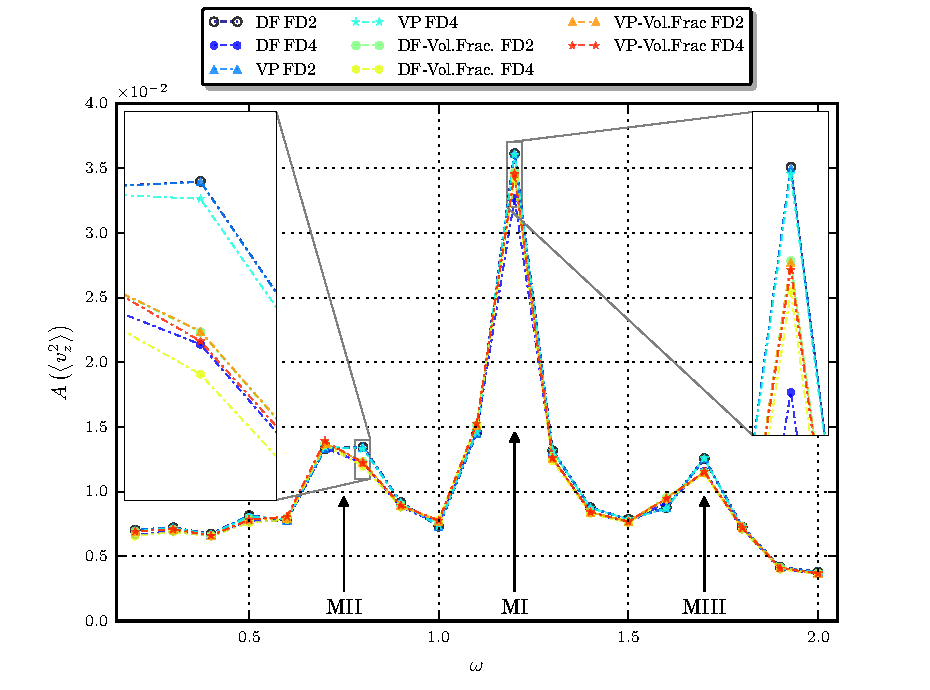
\includegraphics{gfx/cone/cylinder/cylinder.pdf}\label{fig:cone:cyl}
  \caption{blabla}

  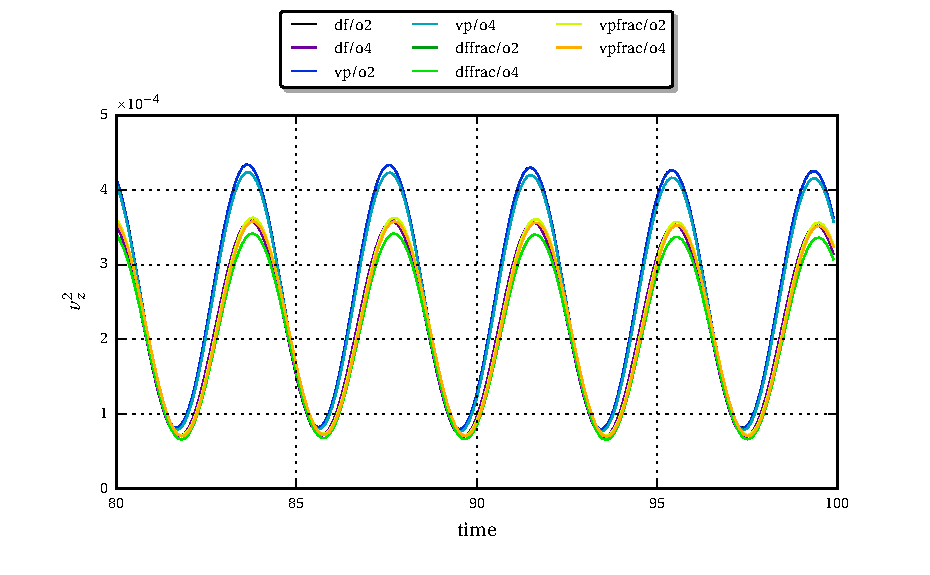
\includegraphics{gfx/cone/cylinder/cyl_vz.pdf}\label{fig:cone:cyl_time}
  \caption{blabla}
\end{figure}
\newpage

-behaviour known theorie
- paper kurz erklären symetrie warum fehlen bestimmte moden ? ?

As a first system we want to investigate the

- erstes test system cylinnder\\
- expectation

- verglein von den bedien implementierungen\\
- first test omega = 1.2 ...\\
- diskussion rand compare to tcflow \\
- test serie verschiede methoden\\
- spektrum dargesstel\\
- evtl raytracer  comparison
- heliziätte dargstellt\\
- results diskussion ip kaputt heli 0 etc \\

\newpage

\section{Simulation of a Liberating Cone}

In this section we will discuss the different numerical simulations, which has been performed
with a liberating cone. We begin with the comparison to the experiment performed by \citep{Beardsley1970}.
As a next step we analyse the physical behaviour when performing the transition from a cylinder
to a cone and finally  we will investigate the influence of different offsets on top of the cone.

\subsection{Simulation of the Experiment}

The setup for this simulation is oriented on the experimental setup given by \citep{Beardsley1970}.
In the experiment a plexiglass cylinder of height $H=\SI{19.95}{\centi\meter}$ and a radius of
$r=\SI{19.95}{\centi\meter}$ was used. The apex half angle was set to $24^{\circ}$ degree.
For the rotation rate a frequency of $\omega =\SI{6.28}{\radian\per\second}$ was chosen.

-boden


As a fluid, water was used, the resulting viscosity,given by \citep{visocisty??}, is $\nu = 1.1$.
The ekman number for this system is given by (KORREKTORLESEN)

\begin{align}
    \Ekman = \frac{\nu}{\Omega (H/2)^2} \approx \frac{\SI{1e-2}{\centi^2\meter\per \second}}{1} \approx 3.2\cdot 1^{-5}
\end{align}


-ekman zahl größer
-winkel anders
-boden cut










\subsection{Results \& Discussion}


\clearpage

\subsection{Transition to from the Cylinder to a Liberating Cone}

 - Close to the ex
first experiment cone
-cone abgebildet nach experiment
- cut spitze bei 0.123123 blabla vgl exp
-setup dargestellt in abbildung bla

\subsection{Results \& Discussion}

\clearpage

\subsection{Liberating Cone with different Offsets at Top}
\subsection{Results \& Discussion}

-description\\
-verfahren und serie\\
-diskussion oberer rand\\
-eigenschaften und influence oberer rand \\


Finally
-nun cone mit und ohne spitze
-teste den einfluss der oberen kante blablabla
-serien vergleich diskussion\
-helizität diskussion\\

In order to test
As a first test

\subsection{Discussion}

\subsection{Numerical Viscosity}
